\section{Layout}

\begin{figure}[!htb]
	\minipage{0.45\textwidth}
		\centering
		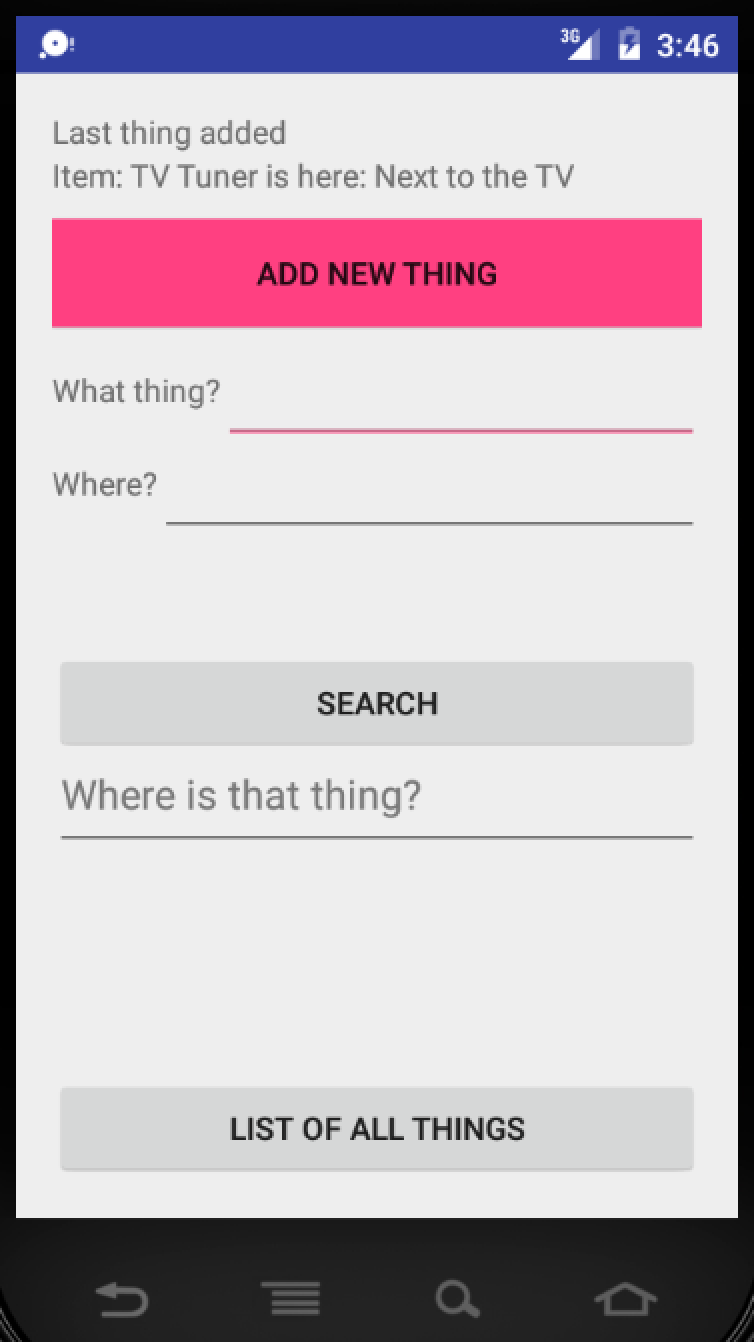
\includegraphics[width=0.9\linewidth]{Tingle-Portrait.png}
		\caption{Portrait view of the main Tingle activity.}
		\label{fig:tingle-view-portrait}
	\endminipage\hfill
	\minipage{0.45\textwidth}
		\centering
		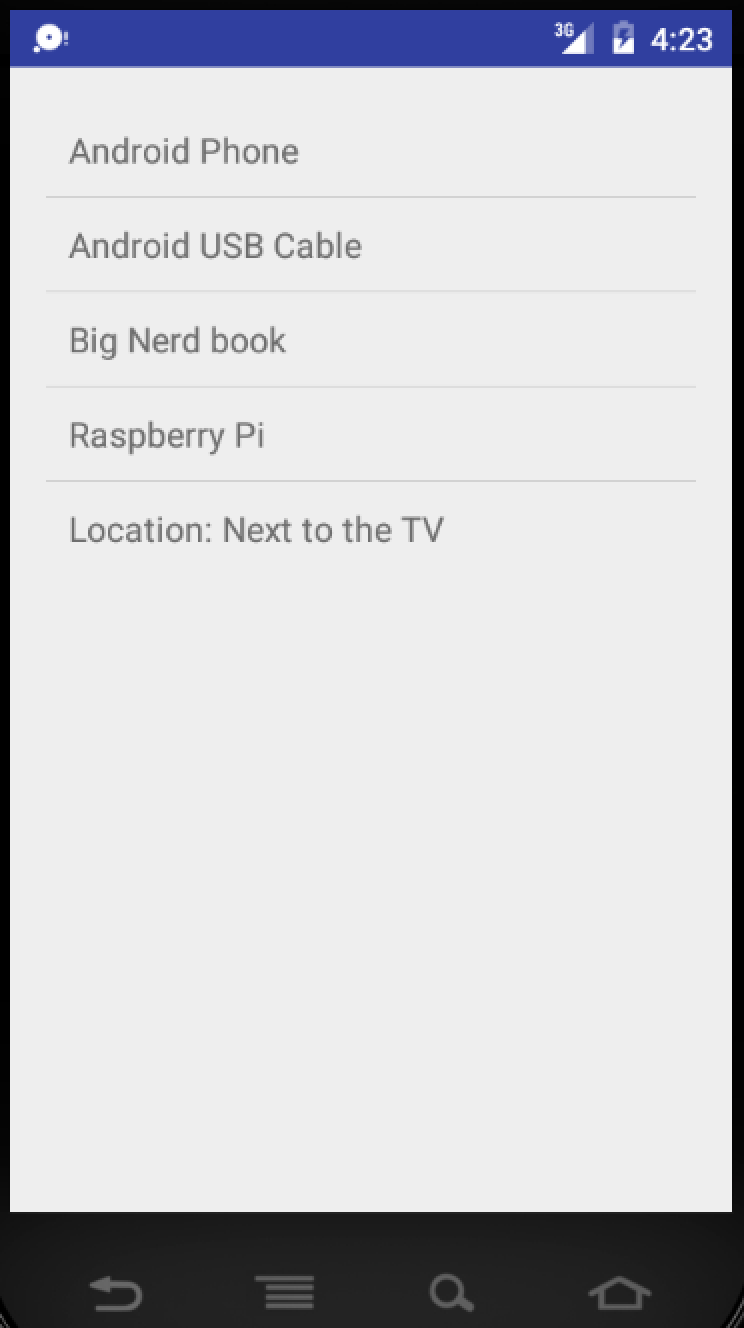
\includegraphics[width=0.9\linewidth]{List-Portrait.png}
		\caption{Portrait view of the main List activity.}
		\label{fig:list-view-portrait}
	\endminipage\hfill
\end{figure}

When running the Tingle App the first view the user sees is shown in Figure \ref{fig:tingle-view-portrait}. In this view the user can add new things and their whereabouts to the database, search for exists things and finally list all things in the database. Clicking the button \texttt{List of all things} will open up the List Activity shown in Figure \ref{fig:list-view-portrait}. The list view is a scrollable list showing all items in the database. Tapping an item in the list will toggle the \emph{What} (i.e the name of the item) and \emph{Where} (the location of the item). The user can also delete an item by Long pressing on an item. A popup dialog appears as seen in Figure \ref{fig:delete-verification-dialog}.

\begin{figure}[H]
	\centering
	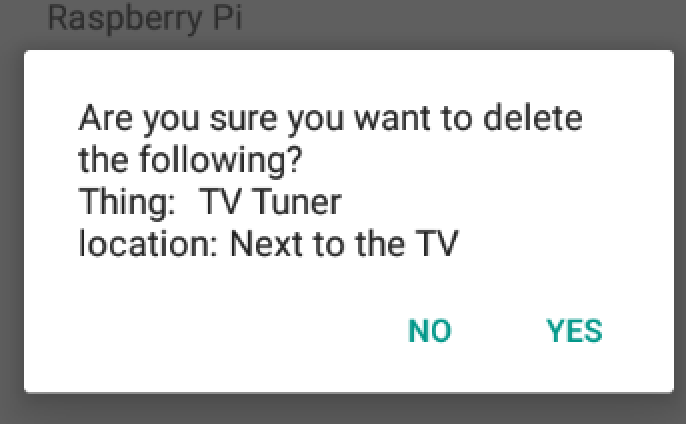
\includegraphics[width=0.3\textwidth]{Longpress-delete-portrait.png}
	\caption{Verification dialog when deleting an item.}
	\label{fig:delete-verification-dialog}
\end{figure}


Changing the orientation to landscape then the two views are show side-by-side. The same functionality applies to this view as they do in portrait mode as described above. The only difference is the removal of the \texttt{List of all things} button since the list is already visible to the right.

\begin{figure}[H]
	\centering
	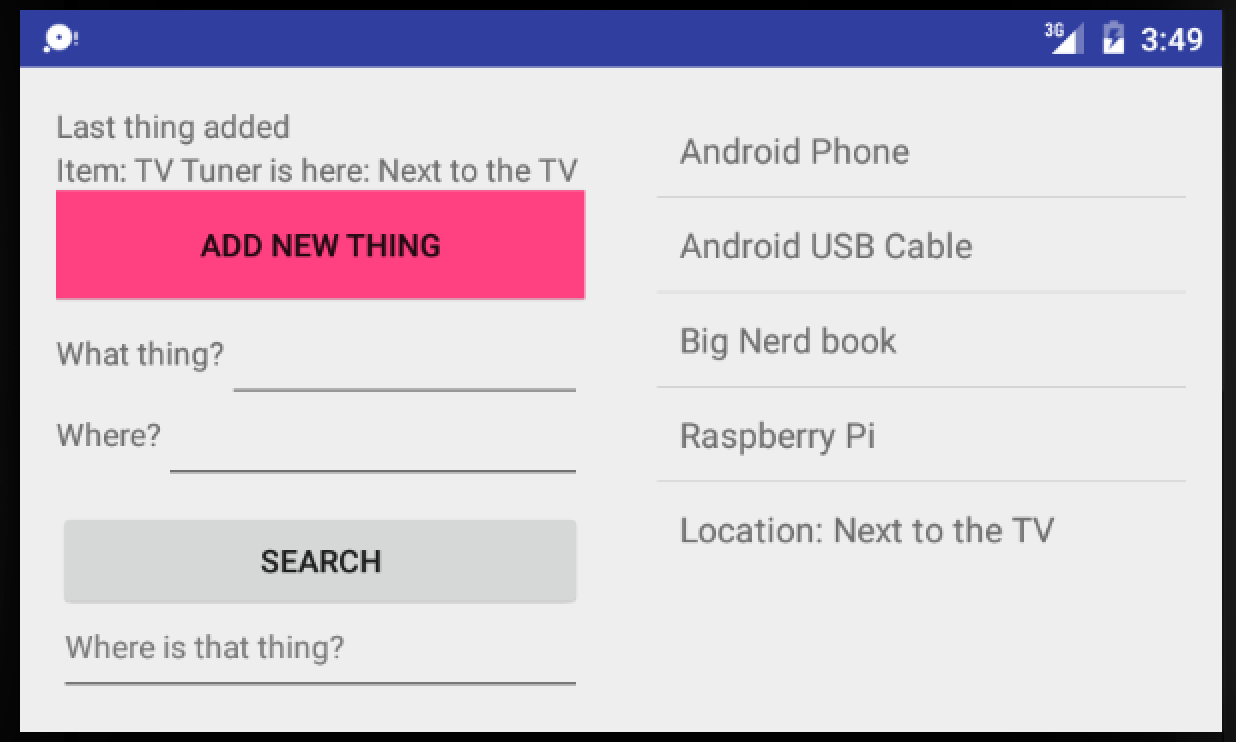
\includegraphics[width=0.6\textwidth]{Landscape-Tap-to-Toggle-Where-and-What.png}
	\caption{Landscape view showing both the main functions as well as the list of things side by side.}
	\label{fig:landscape-main-view}
\end{figure}

\section{Design}


\section{Extensions }


\section{Testing}
The testing of the App has been separated into two four different parts. One for each view and one for each orientation of the device. 

\begin{figure}[H]
	\renewcommand*{\arraystretch}{1.5} % Redefine padding size
	\begin{tabular}{| c | p{3.5cm} | p{3.5cm} | p{3.5cm} |}
		\hline
		{\textbf{ID} } & {\textbf{Test Case} } & {\textbf{Expected Output}} & {\textbf {Actual Output}} \\\hline\hline
		% -- test 1
		A & Running the App opens up the Tingle view & The Tingle view is shown & The Tingle view is shown  \\ \hline
		% -- test 2
		B &	Clicking the \texttt{List of All Things} button in the Tingle view opens up a the List view. & The List view is shown. & The List view is shown. \\ \hline
		C & It is possible to add an item to the database. & An item is successfully added to the database. & An item is successfully added to the database. \\ \hline
		D & It is possible to search for an item in the database. & A Toast is displayed showing the location of the found item. & A Toast is displayed showing the location of the found item. \\ \hline
	\end{tabular}
	
	\caption{Test cases of the Tingle view in Portrait mode.}
	\label{tab:test-cases-tingle-portrait}
\end{figure}

\begin{figure}[H]
	\renewcommand*{\arraystretch}{1.5} % Redefine padding size
	\begin{tabular}{| c | p{3.5cm} | p{3.5cm} | p{3.5cm} |}
		\hline
		{\textbf{ID} } & {\textbf{Test Case} } & {\textbf{Expected Output}} & {\textbf {Actual Output}} \\\hline\hline
		% -- test 1
		A & Running the App opens up the Tingle view & The Tingle view is shown & The Tingle view is shown  \\ \hline
		% -- test 2
		B &	Clicking the \texttt{List of All Things} button in the Tingle view opens up a the List view. & The List view is shown. & The List view is shown. \\ \hline
		C & It is possible to add an item to the database. & An item is successfully added to the database. & An item is successfully added to the database. \\ \hline
		D & It is possible to search for an item in the database. & A Toast is displayed showing the location of the found item. & A Toast is displayed showing the location of the found item. \\ \hline
		E & & & \\ \hline
	\end{tabular}
	
	\caption{Test cases of the Tingle view in Landscape mode.}
	\label{tab:test-cases-tingle-landscape}
\end{figure}


\section{Issues}


Code duplication using the Activities.

I could make a common file with the side-by-side fragment layout and programatically test
if we are in landscape orientation.